\section{Implementation Details}

This section describes implementation details of the proposed solution. 
It highlights key aspects of the core implementation, OpenCL specifics, optimization of particular operations, and high-level optimizations of graph algorithms.

\subsection{Core}

The implemented library uses the concept of a registry to find operations as shown in Fig.\ref{fig:reg}. A call to a particular operation is stored as a command to be executed later by \textit{Dispatcher}. For each command the special lightweight string key is built depending on type of the operation and arguments passed. This key is used as a regex to get the required implementation of the requested operation. The advantages of the proposed approach are listed below.

\begin{itemize}
    \item \textit{Late binding}. The operation call becomes a command. The processing of such a command can be configured at run time. Changing the acceleration backend can be done without recompilation. Moreover, several backends can be transparently used within a single application.
    \item \textit{Optionality of accelerator}. The acceleration backend is free to support only those operations that require it. Fallback implementations will be used automatically for the rest of the operations.
    \item \textit{Performance tuning}. The key of the command reflects operation type, arguments types, passed user functions types, etc. It can be used for \textit{ad-hoc} optimizations. Custom operation implementation with a verbose key can be also stored in the registry. If several operations match the key, the longest key is used, since it is more specific for a particular operation.
    \item \textit{Scheduling}. The full list of submitted commands for execution can be examined at runtime. This opens up the possibility for the fusion of some operations, sorting, rearrangement, and any other high-level optimizations that require introspection.
\end{itemize}

\begin{figure}[]
\centering
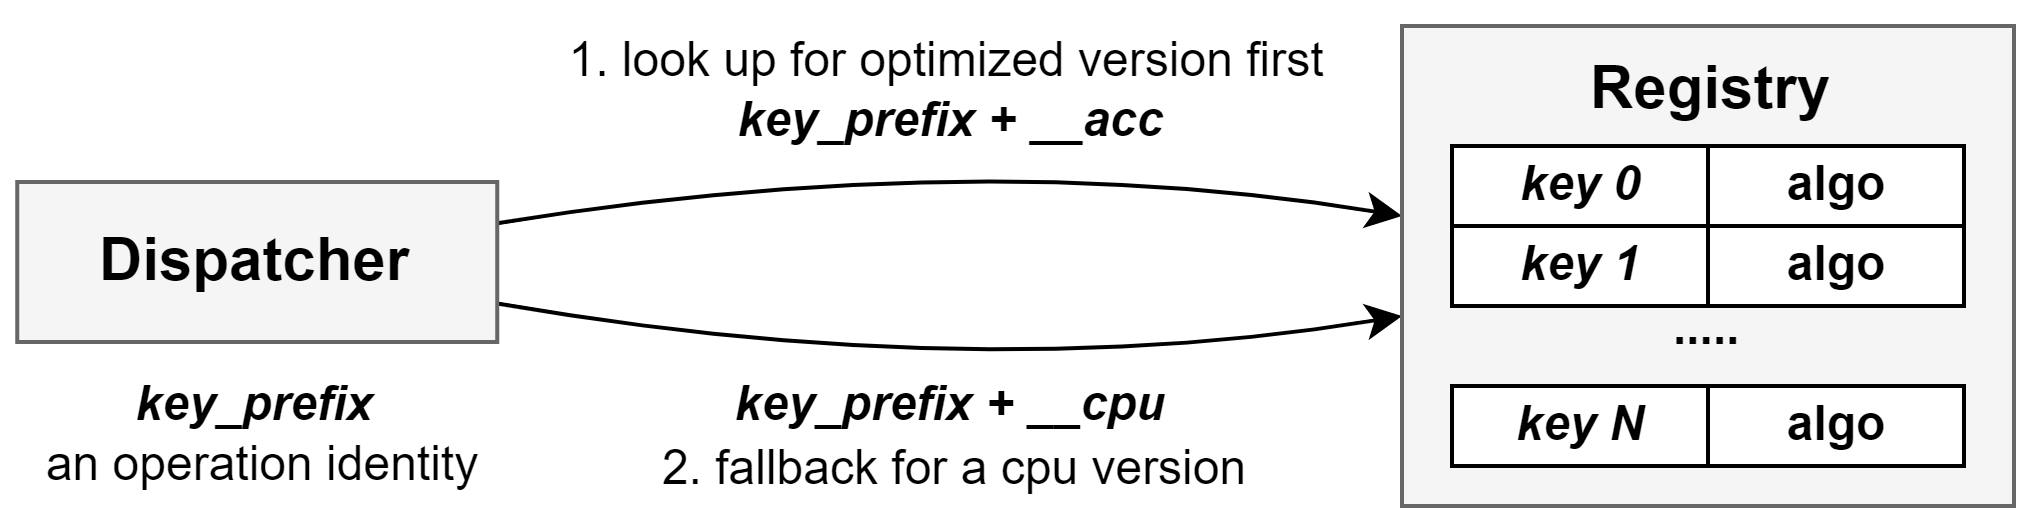
\includegraphics[width=0.95\linewidth]{figures/registry.png}
\caption{Registry of operation implementations. Keys with special syntax used to fetch required operation in a specific order at runtime.}
\label{fig:reg}
\end{figure}

\subsection{OpenCL}

OpenCL 1.2 is used as the primary API for backend GPU implementation. Header files with C and C++ definitions are supplied with the source code of the project. Official Khronos installable client driver (ICD) loader bundled within a library to load at runtime particular OpenCL implementation depending on running OS and GPU vendor. 

Implementation of sparse linear algebra algorithms for a GPU requires auxiliary libraries for memory management, sorting, reducing, merging, scanning, etc. 
Nvidia Cuda platform features libraries such as Thrust and Cub.  
OpenCL lacks such support. All primitives for this project are implement from a scratch in most cases. What is an extra challenge. Third-party library, such as Boost Compute~\cite{10.1145/2909437.2909454:boost:compute}, cannot be used, since it has significant runtime overhead, portability and performance issues, and lack of long term support.

User-defined functions for GPU usage are represented as strings with additional metadata, such as type of parameters, return types, unique id, etc. 
Source code of particular operations stored in a form of .cl files. 
Operations implemented with generalization for parameters types and user functions. 
Their definitions obtained later at runtime in a compilation step through the text pre-processing.
Compilation of actual OpenCL kernels is done on demand. 
All compiled kernels are stored in a cache. Cache key is composed from types of kernel parameters, defines, etc., which identify uniquely a particular variation of a kernel. 
Key composition is done in O(1). In-place allocation is utilized for a key builder to avoid global heap usage. 
In order to reduce CPU overhead and keep access to the cache fast, library uses robin hood hashing based hash map. 

Custom linear memory allocator implemented in order to reduce the overhead of frequent and small buffer allocations, arising in a time of execution of some operations. Allocator uses sub-buffer mechanism and serves request typically less than 1 MB of size. Otherwise, the general GPU heap is used.

\subsection{Linear Algebra Operations}

The following primitives are the core of computations: \textit{masked sparse-vector sparse-matrix product}, \textit{masked sparse-matrix dense-vector product} and \textit{masked sparse-matrix sparse-matrix product}. Efficient implementation and load balancing of those operations dominate the performance of particular algorithms. The following paragraphs give an insight into these operations implementation in the library.

\textit{Masked sparse-vector sparse-matrix product}. The implementation is based on the algorithm proposed by Yang et al.~\cite{7284398:spvspm}. It is a \textit{k}-way merge based algorithm which suites well for sparse vectors. Our implementation uses custom gather to collect temporary products. Radix sort used to sort products for further reduction. Reduction by key uses parallel prefix scan to carry out final destination of reduced values.

\textit{Masked sparse-matrix dense-vector product}. The implementation of this operation relies on a classic row-based parallel algorithm. Both scalar and vector versions are implemented to fit better relatively sparse and dense matrix rows. 

\textit{Masked sparse-matrix sparse-matrix product}. The implementation of this algorithm uses the approach proposed by Yang et al.~\cite{yang2019graphblast}. It is straightforward single-pass row-major and column-major matrix product. Mask is used to estimate the size of the final result to filter out some result of the product. 

\subsection{Graph Algorithms}

The advantage of the linear algebra approach is that graph algorithms can be easily composed of primitive operations using a few lines of code. For preliminary study breadth-first search (BFS), single-source shortest paths (SSSP), page rank (PR) and triangles counting (TC) algorithms were chosen. These are the most commonly evaluated graph algorithms. They allow one to test basic operations and key aspects of graph frameworks performance. Implementation details for chosen algorithms are given below. 

\textit{BFS}. It utilizes a number of optimizations described by Yang et al.~\cite{https://doi.org/10.48550/arxiv.1804.03327:pushpull}. It uses masking to filter out already reached vertices, change of direction (push-pull) to switch from sparse from to dense and vice versa, and early exit in \textit{mxv} operation.

\textit{SSSP}. This algorithm uses change of direction as well. Also, it employs filtering of unproductive vertices according to Yang et al.~\cite{yang2019graphblast}. Vertices which do not relax their distance in current iteration are removed from a front of the search. It keeps workload moderate. 

\textit{PR}. This algorithm assigns numerical weights to objects in the network depending on their relative relevance. As a key operation it uses \textit{mxv} operation with a dense vector. For error estimation it uses custom element-wise function with a fusion of subtraction and square operations.  

\textit{TC}. Triangles counting uses masked sparse matrix product~\cite{yang2019graphblast} and reduction. As an input algorithm accepts a lower triangular component $L$ of an adjacency matrix of the source graph. The result is a count of non-zero values from $B = LL^T .* L$, where $.*$ used for the masking. The second argument is not actually transposed, since row-column based product gives exactly the required effect.